\chapter{Arbeitspunkt-Regelung}\label{cha:apr}

In diesem Kapitel wird die Modellierung des Gesamtsystems erläutert und auf dessen Implementierung in Simulink eingegangen.

\section{Einleitung}%\label{sec:}



\section{Aufbau in \Simulink}



\section{Implementierung in \Matlab}



\section{Anfangswert-Tests}

\begin{figure}
	\centering
	\begin{minipage}[t]{0.45\linewidth}
		\centering
		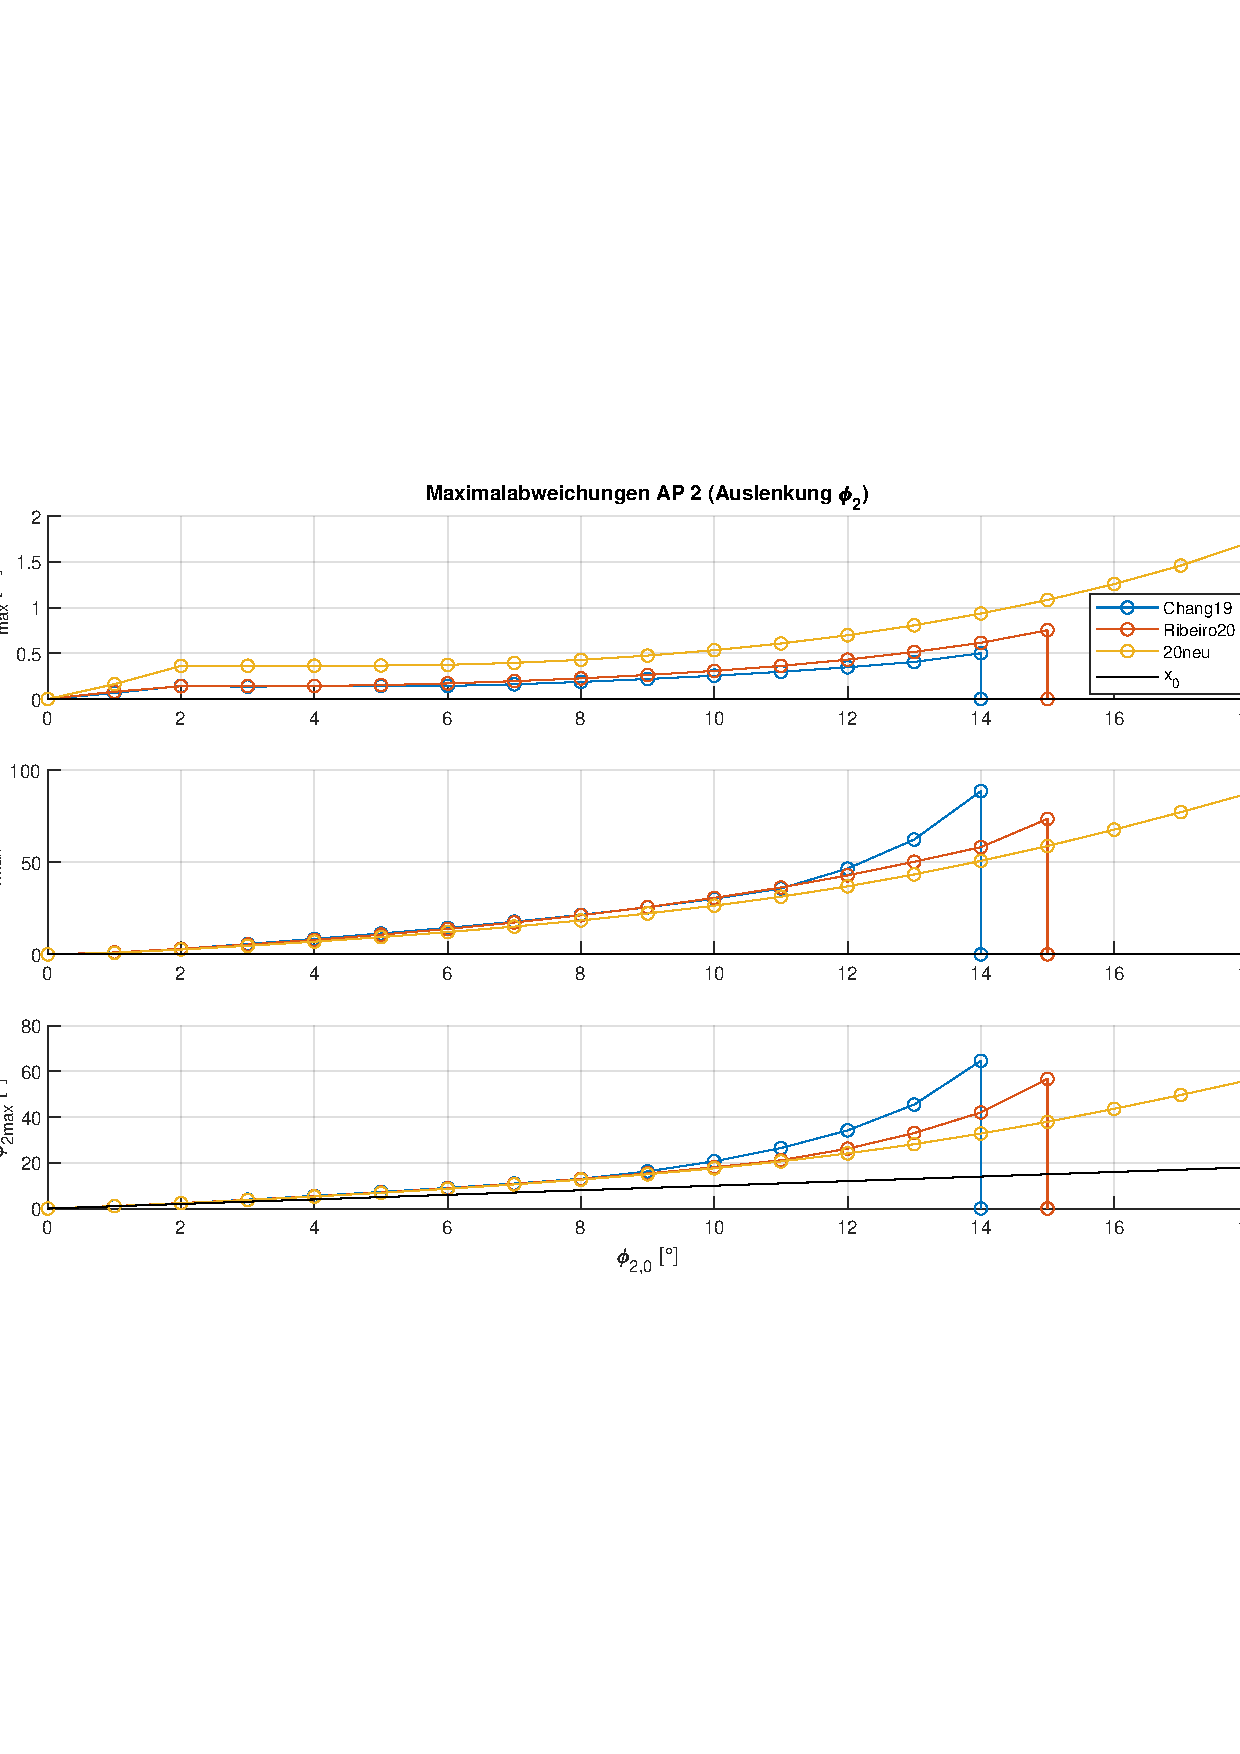
\includegraphics[scale=0.5]{Bilder/Parameter neu (Ribeiro) Creg off/AP2.pdf}
		%\caption{\ap  2}
		\label{fig:ap2}
	\end{minipage}
	\hfill
	\begin{minipage}[t]{0.45\linewidth}
		\centering
		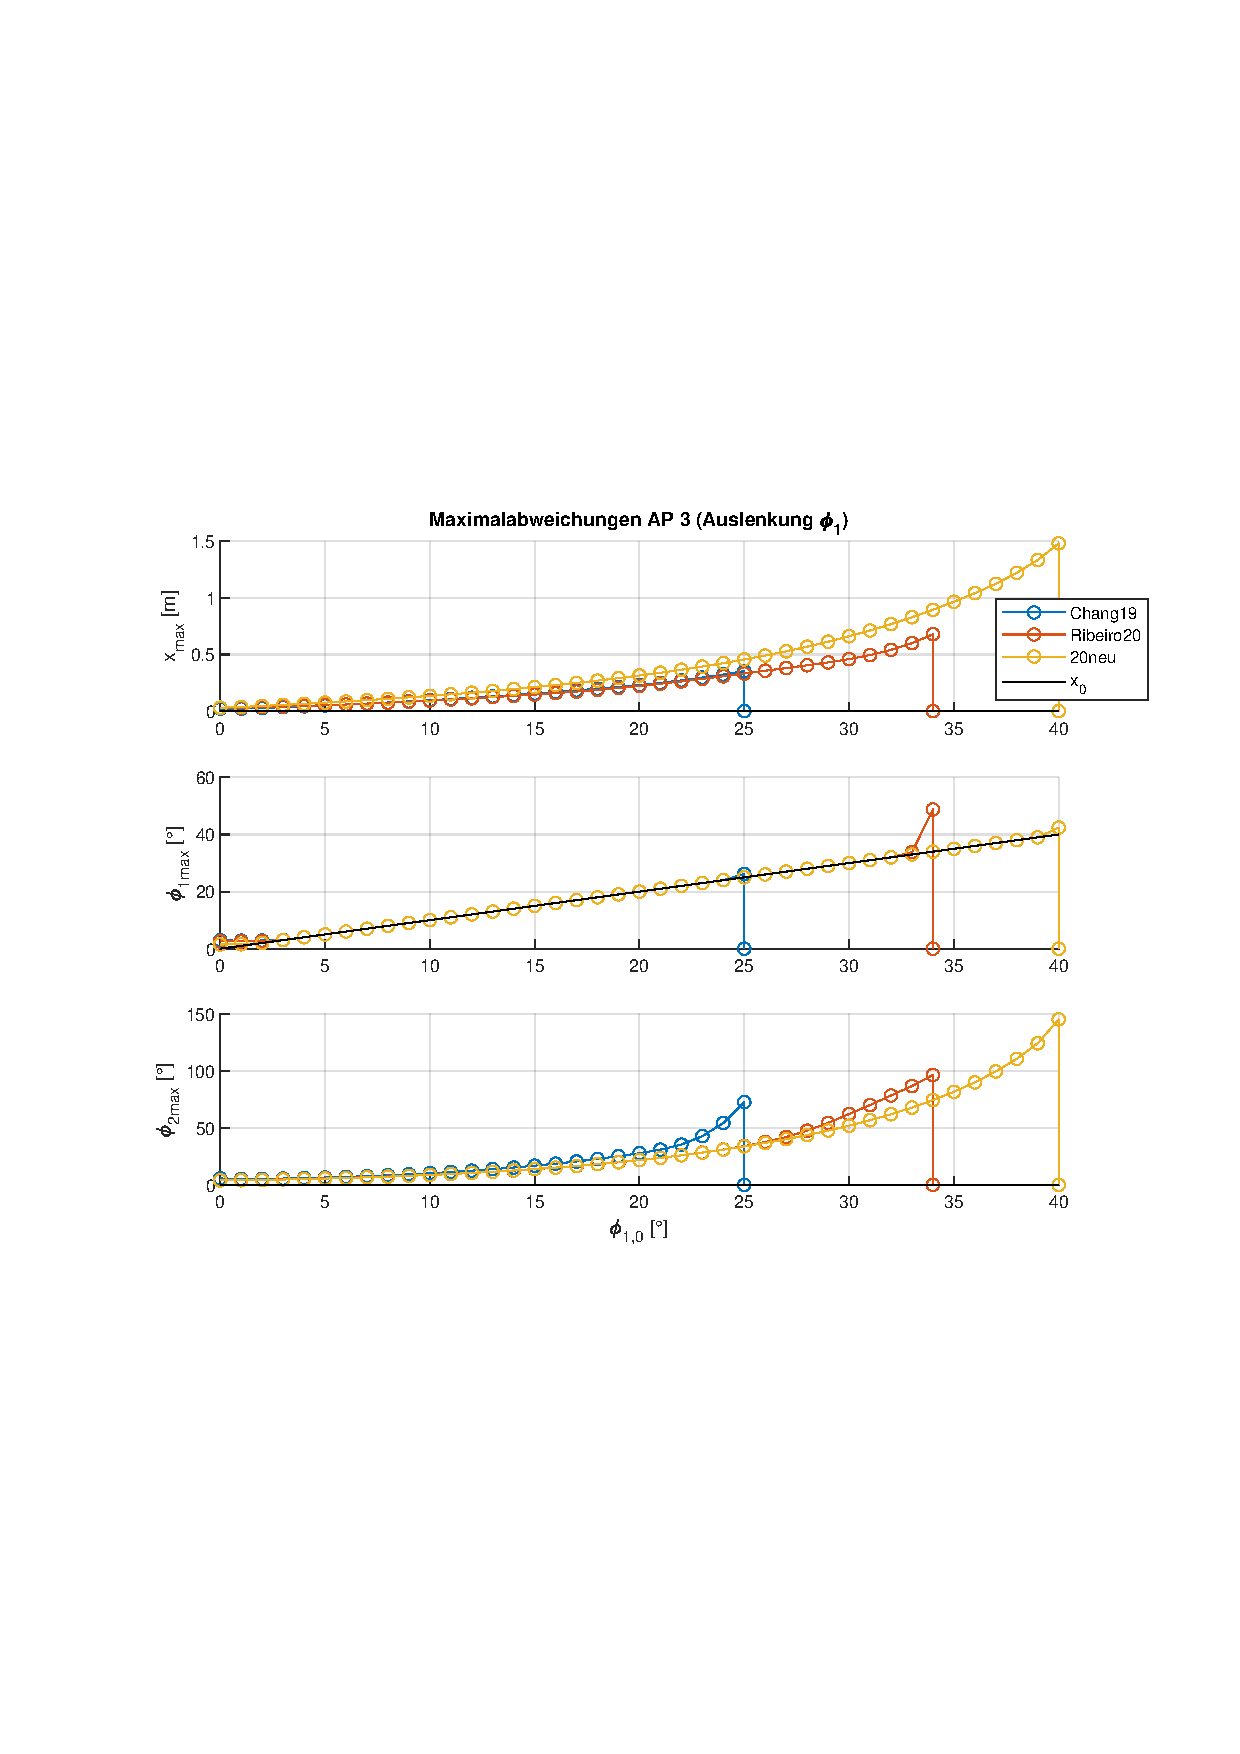
\includegraphics[scale=0.5]{Bilder/Parameter neu (Ribeiro) Creg off/AP3.pdf}
		%\caption{\ap  3}
		\label{fig:ap3}
	 \end{minipage}
	\\
	\begin{minipage}[t]{0.45\linewidth}
		\centering
		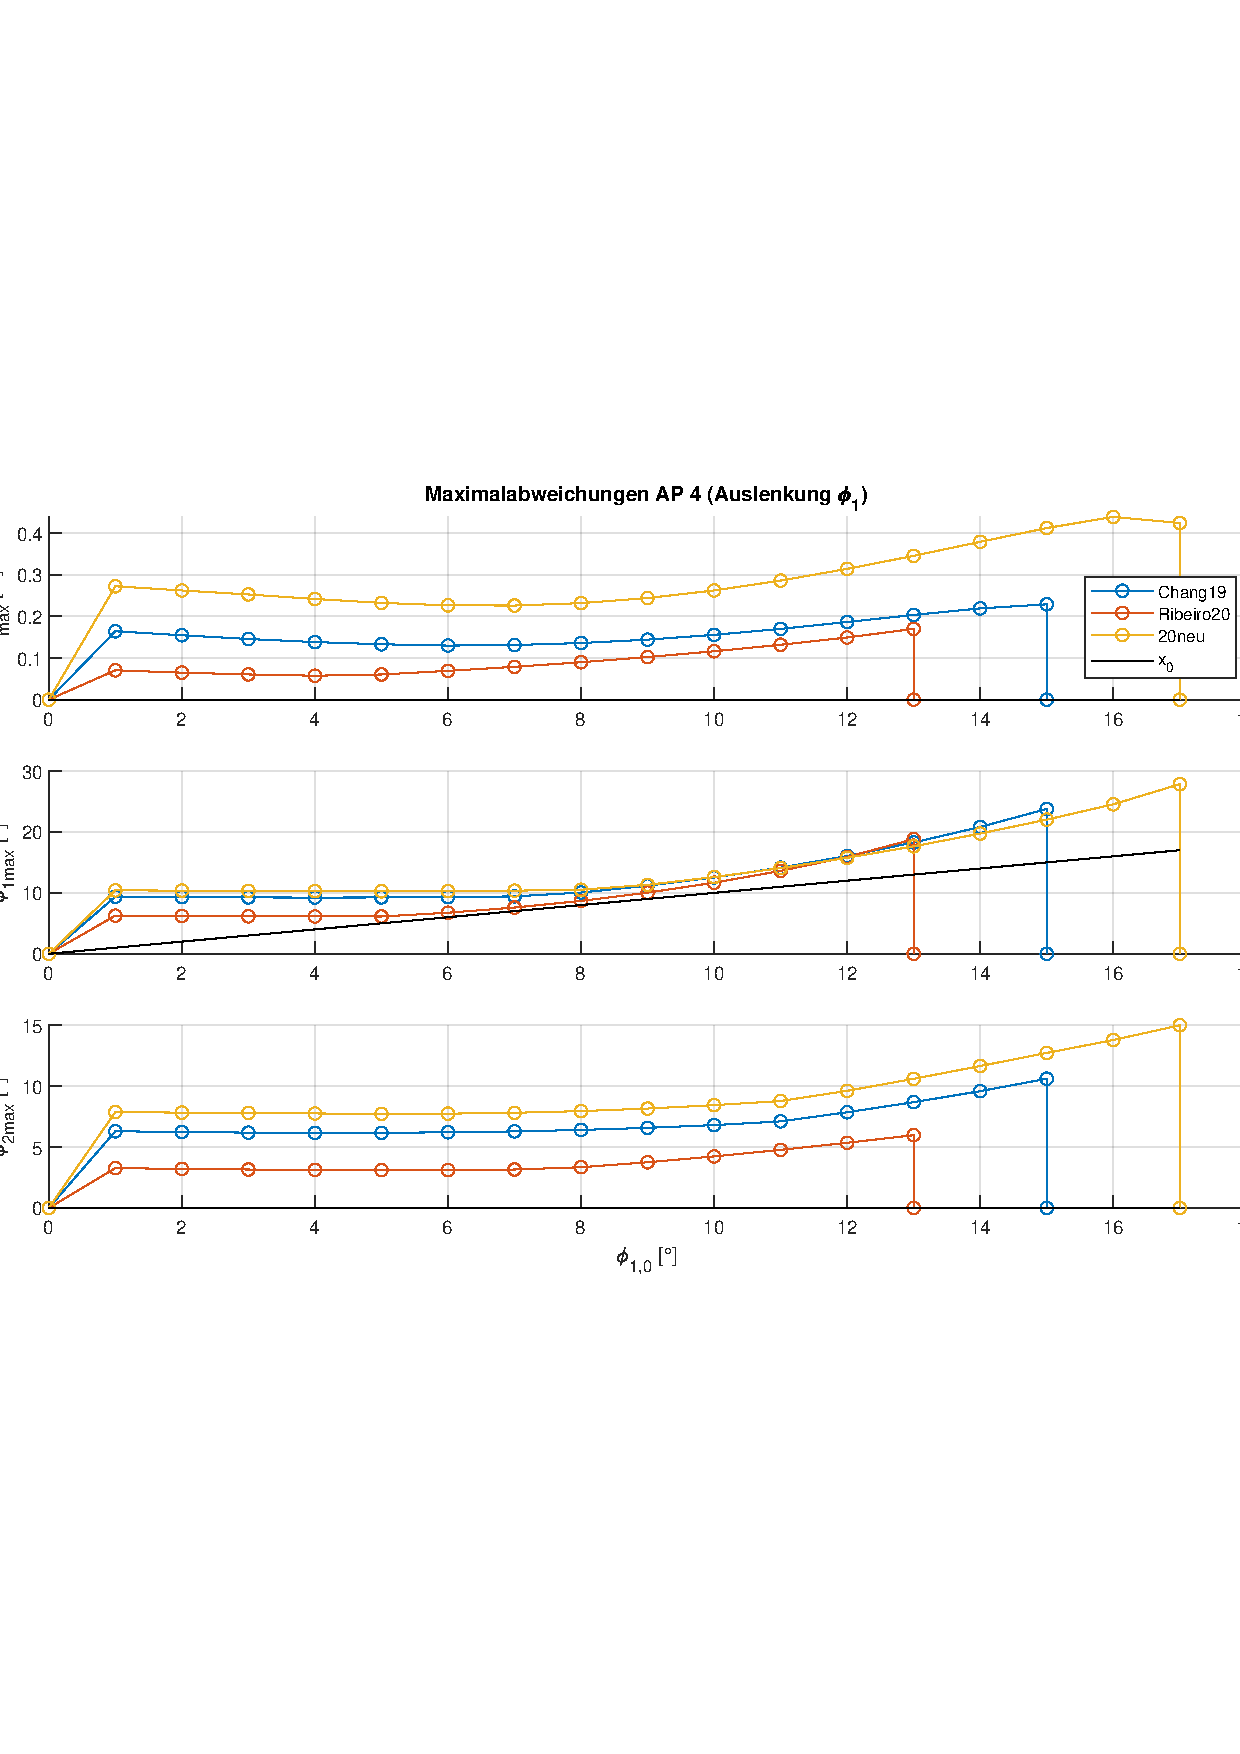
\includegraphics[scale=0.5]{Bilder/Parameter neu (Ribeiro) Creg off/AP41.pdf}
		%\caption{\ap  3}
		\label{fig:ap3}
	 \end{minipage}
	\hfill
	\begin{minipage}[t]{0.45\linewidth}
		\centering
		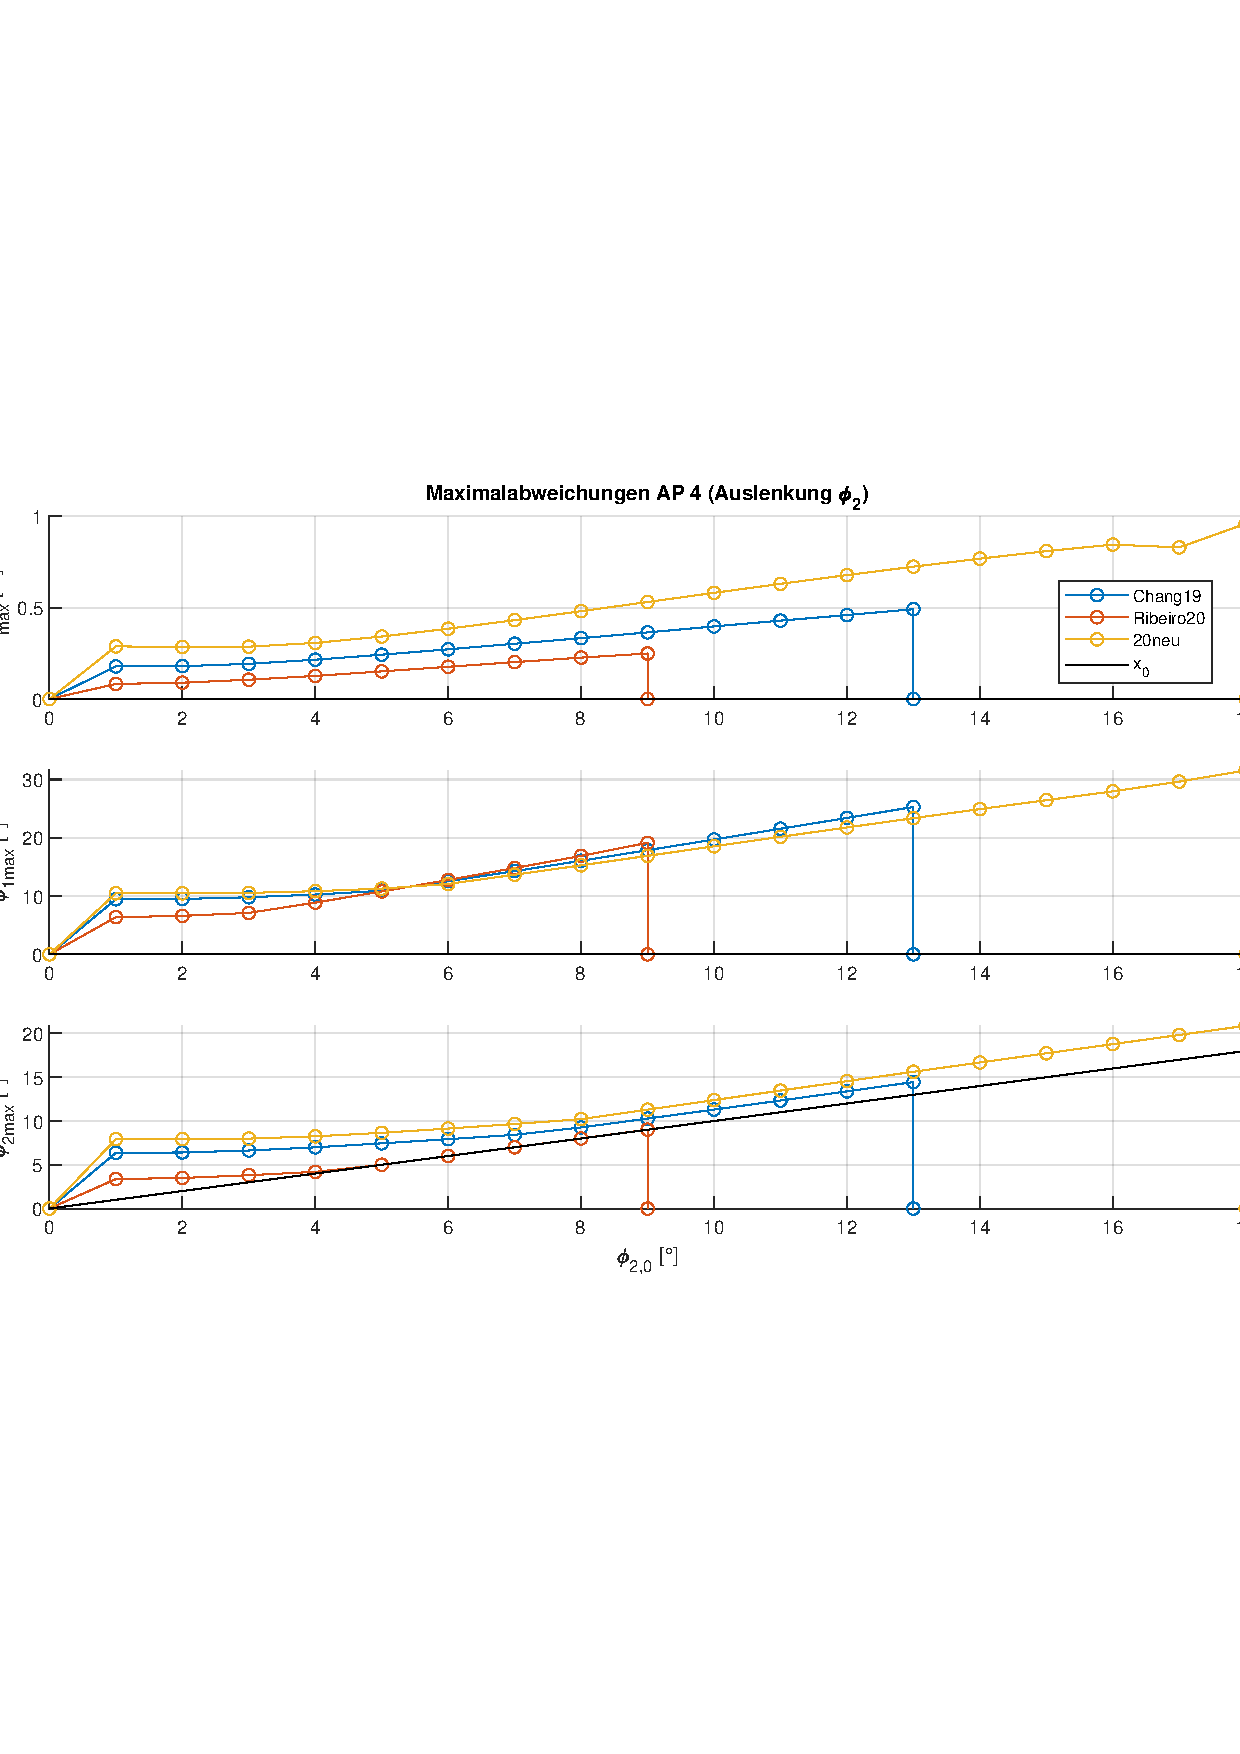
\includegraphics[scale=0.5]{Bilder/Parameter neu (Ribeiro) Creg off/AP42.pdf}
		%\caption{\ap  3}
		\label{fig:ap3}
	 \end{minipage}
	\caption{Vergleich QR-Parameter (System Ribeiro)}
%\vspace{15pt}
\end{figure}




\section{QR Parameter Tests}



\section{System Parameter Tests}



